\documentclass[10pt,a4paper]{article}
\usepackage[utf8]{inputenx}
\usepackage{cmap} 
\usepackage[T1]{fontenc}
\usepackage[english]{babel}
\usepackage[top=3cm,bottom=3cm,outer=3.2cm,inner=3.2cm]{geometry}
\usepackage[backend=biber,sortcites=true,doi=false,url=false,firstinits=true,hyperref,maxbibnames=9,maxcitenames=3,sorting=nyt]{biblatex}

\addbibresource{refs.bib}
\usepackage{csquotes}
\usepackage{url}
\usepackage{hyperref}
\usepackage{amsfonts}
\usepackage{amssymb}
\usepackage{amsthm}
\usepackage{mathtools}
\usepackage{dsfont}       %Stroke Fonts for Number Sets
\usepackage{cases}

\def\Pset{\mathcal{P}}
\def\Sset{\mathcal{S}}

\begin{document}
\title{Perprof-py: a {P}ython package for performance profile}
\author{Raniere Gaia Costa da Silva\thanks{IMECC/Unicamp.} \and Abel Soares Siqueria\thanks{IMECC/Unicamp}  \and Luiz-Rafael Santos\thanks{IMECC/Unicamp}}
\date{Technical Report \\ Operational Research and Optimization Laboratory (LPOO) \\ IMECC/Unicamp \\ Campinas, Brazil \\ \today}
\maketitle

\begin{abstract}
Benchmarking optimization packages are very important in optimization field,
not only because it is one of the ways to compare solvers, but also to uncover
deficiencies that could be overlooked while one is developing a new solvers. During
benchmarking, one can obtain a large amount of  informations, like CPU time, number of functions
evaluations, number of iterations and much more. These informations, if presented
as tables, can be difficult to be analyzed, due, for instance, to large amount of data.
Therefore, researchers started testing and developing tools to better process and understand optimization benchmark 
data. One of the most widespread tools is \emph{ Performance Profile} graphics
proposed by \textcite{Dolan:2002du}. In this context, we implemented a free software that makes Performance Profile using data provided by user in a friendly manner. This software produces graphics in PDF using \LaTeX with PGF/TikZ~\cite{TikZ} and \texttt{pgfplots}~\cite{pgfplots} packages, in PNG using \texttt{matplotlib}~\cite{Hunter:2007}
and can also be easily extended to use with other plot library. The software is
implemented in Python3 with support for internationalization. %and is available on \url{https://github.com/lpoo/perprof-py}.

\textbf{Keywords:} Software benchmarking. Performance profile. Python.
\end{abstract}

\section*{Introduction} 

The Performance Profile of a solver is the cumulative distribution
    function of a performance metric, e.g., CPU time, number of functions
    evaluations, number of iterations, or others, that we will call \emph{cost}.

    Given a set $\Pset$ of problems and a set $\Sset$ of solvers, for each problem $p
    \in \Pset$ and solver $s \in \Sset$, we define $t_{ps}$ as the cost
    required to solve problem $p$ by solver $s$ and
    \begin{align*}
      r_{ps} = \frac{t_{ps}}{\min\{t_{ps}: s \in S\}}
    \end{align*}
    as the performance ratio of solver $s$ for the problem $p$ when compared
    with the best performance by any solver on this problem.

    \textcite{Dolan:2002du} defines the probability for solver $s \in \Sset$ to solve one
    problem within a factor $\tau \in \mathds{R}$ of the best performance
    ratio as the function
    \begin{align*}
      \rho_s(\tau) = \frac{| \{p \in \Pset: r_{ps} \leq \tau\} |}{| \Pset |}
    \end{align*}
     For a given $\tau$, the best solver is the one with the highest
    value for $\rho_s(\tau)$.

    EXPLAIN WHY WE WANTED TO DEVELOP PERPROF-PY

\section*{Implementation and architecture}
How the software was implemented, with details of the architecture where relevant. Use of relevant UML diagrams may be appropriate. Please also describe any variants and associated implementation differences.

\section*{Quality control }
Detail the level of testing that has been carried out on the code (e.g. unit, functional, load etc.), and in which environments. 

\section*{(2) Availability }

\paragraph*{Operating system}
Please include minimum version compatibility.

\paragraph*{Programming language}
Please include minimum version compatibility.

\paragraph*{Additional system requirements}
E.g. memory, disk space, processor, input devices, output devices.

\paragraph*{Dependencies}
E.g. libraries, frameworks, incl. minimum version compatibility.

\paragraph*{List of contributors}
Please list anyone who helped to create the software (who may also not be an author of this paper), including their roles and affiliations.

\paragraph*{Software location:}
Archive (e.g. institutional repository, general repository) (required) 

Name: The name of the archive

Persistent identifier: e.g. DOI, handle, PURL, etc.

Licence: Open license under which the software is licensed

Publisher: Name of the person who deposited the software

Date published: dd/mm/yy

Code repository (e.g. SourceForge, GitHub etc.) (optional) 

Name: The name of the code repository

Identifier: The identifier (or URI) used by the repository 

Licence: Open license under which the software is licensed

Date published: dd/mm/yy

Emulation environment 

Name: The name of the emulation environment

Identifier: The identifier (or URI) used by the emulator

Licence: Open license under which the software is licensed here

Date published: dd/mm/yy

Language

Language of repository, software and supporting files




\printbibliography
\end{document}


  \begin{posterbox}[column=0,below=auto,name=perprof]{perprof-py}
    We implemented a free/open software that generates performance profiles using data
    provided by the user in a friendly manner. This software produces graphics in PDF
    using LaTeX with PGF/TikZ and pgfplots packages,
    in PNG using matplotlib and can also be easily extended to
    use other plot libraries. The software is implemented in Python3 with
    support for internationalization and is available at
    \url{https://github.com/lpoo/perprof-py} under GPLv3 license.
  \end{posterbox}

  \begin{posterbox}[column=1]{Features}
    Some of perprof-py features are:
    \begin{itemize}[noitemsep]
      \item high quality output (in more than one format);
      \item lots of native options/filters;
      \item input processing to limit solver minimum and maximum costs and set
        of problems;
      \item native internationalization support.
    \end{itemize}

    \begin{center}
      \begin{tabular}{cc}
        \includegraphics[width=0.45\linewidth,height=108pt]{abc-bw-semilog.pdf} &
        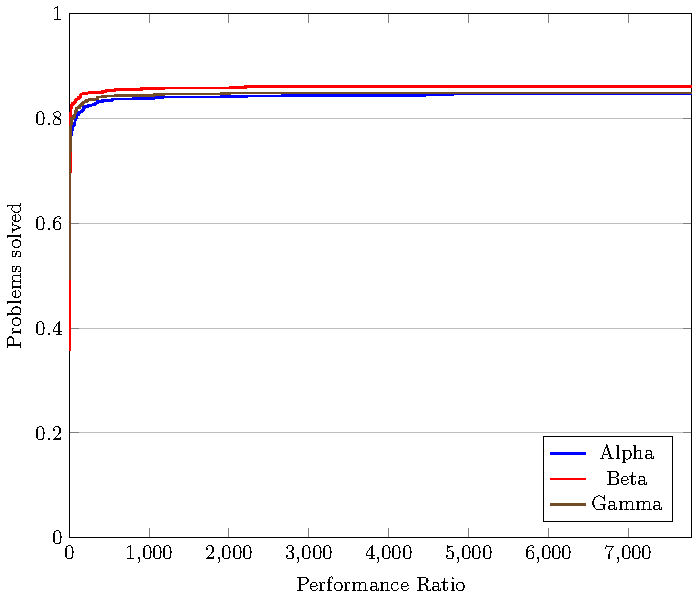
\includegraphics[width=0.45\linewidth,height=108pt]{abc.pdf} \\
        Black and white & Linear scale \\
        \includegraphics[width=0.45\linewidth,height=108pt]{abc-100.pdf} &
        \includegraphics[width=0.45\linewidth,height=108pt]{abc-hs.pdf} \\
        Performance ratio limit & Subset (Hock-Schittkowski)
      \end{tabular}
    \end{center}

    Besides the previous features, the package can be easily used in a range
    of external tools that support Python.
  \end{posterbox}

  \begin{posterbox}[column=1,below=auto]{Input file}
    Each solver to be used in the benchmark must have a file like:

    \begin{lstlisting}
YAML information
Problem01 exit01 time01
Problem02 exit02 time02
    \end{lstlisting}

    In the YAML information you can set the name of the solver, and some
    flags for perprof-py.
    Each line beyond that has 3 columns that mean, in order:
    \begin{itemize}[noitemsep]
      \item The name of the problem;
      \item Exit flag;
      \item Elapsed time.
    \end{itemize}
  \end{posterbox}

  \begin{posterbox}[column=1,below=auto]{Future works}
    Some of our next improvements consist of:
    \begin{itemize}[noitemsep]
      \item add metadata support and also support data profiles as defined by
        \textcite{More2009};
      \item add support for the analysis of the objective value, and the primal and
        dual infeasibilities;
      \item add more backends and more output formats.
    \end{itemize}
  \end{posterbox}

  \begin{posterbox}[column=1,below=auto]{References}
    \printbibliography[heading=none]
  \end{posterbox}

  \begin{posterbox}[column=0,span=2,below=auto,height=bottom,
    boxshade=none,textborder=none,headerborder=none,headershade=plain,
  headerColorOne=bgcolor2, boxheaderheight=0cm]{}
  \begin{center}
    \begin{tabular}{cl}
      \multirow{3}{*}{\includegraphics[height=24pt]{figures/cc-by}} & \\
                                                                    & \Large
      This work is licensed under a
       Creative Commons Attribution 3.0 Unported License.
    \end{tabular}
  \end{center}
  \end{posterbox}
\end{poster}
